\chapter{Results}

This chapter goes through the full process of making, training and testing the \gls{gnn} step by step, from first iterations of the very simple model to more fine tuned models and other methods that were tested. Reasoning and explanations for the choices and changes made during the process are also given along the way. Finally, best results that were achieved are presented. 

\section{Progress}

\subsection{Experimenting environment}

The experiments have been done on a computer equiped with 11th Gen Intel(R) Core(TM) i7-11700K 3.60GHz 8-core CPU, 16 GB RAM and NVIDIA RTX 3080Ti graphics card. All the code for the \gls{gnn} model was written in Python using Pytorch Geometric (PyG) library \cite{pytorchlib}.

\subsection{Simple line graph model}

The first step was to try the simplest line graph model with most of the hyperparameters set to default and train it on a smaller scale using a small subset of 1000 graphs from the MNIST dataset, training it for 100 iterations and then evaluating its performance on 100 graphs from the evaluation dataset. The performance is evaluated based on the total weight of the edges in the solution set compared to the greedy algorithm and the optimal if the results are close enough. Before using a large dataset that may take some time to process, it is worth confirming that the model works as intended. One also does not want to add complexity to the model without any reason. An unnecessary large and complex model affects the running time and has a higher chance of overfitting. 

The first model had two layers with 64 neurons each. Remember that in a line graph every node represents an edge in the original graph. The first problem encountered was due to the majority of line graph nodes not being included in the matching. The model learned to set all nodes to be dropped and still get a rather high accuracy score, since the accuracy is measured by correctly classifying the nodes and not the total weight the classification produces. This was resolved by adding class weights as a parameter for the Adam optimizer during training. Class weights tell the model how important each class is, where the two possible classes stand for belonging to the solution and not. After testing the class weight distribution by increments of 0.1, the most effective result was achieved by assigning the nodes that are in the matching a value of 0.9 and the ones that are not 0.1. The problem seemed to be resolved, and the model's output was no longer one-sided. The model resulted on average with 55\% of optimal weight possible when the tested on 100 graphs from the validation dateset. This was an expected result considering the small size of the current training dataset, but it at least showed that the model is gaining some knowledge compared to an untrained model, as well as a solution that randomly picks edges, where both resulted in 50-51\% of the optimal solution. 

The next step was to experiment with the learning rate parameter for the optimizer. The learning rate is used to decide by how much the models' weights are adjusted after each iteration. The high learning rates resulted in unstable training with information loss jumping too much, which indicated that the model made overly large adjustments after each training iteration. The low learning rates did not give enough progress and made the training process too slow. The default value of 0.001 worked well as a middle ground, leaving the best result so far unchanged at 55\%.

A model that barely outperforms a random solution is not very useful. Poor performance at this point was expected since the goal was to test if the model worked as expected and given a very limited training dataset. However, before adding more data and prolonging training, we can experiment with some of the parameters of the network to see if they make any impact.

\subsection{Model improvements and data augmentation}

At this stage, the model seemed to slowly improve and learn. Even with the current limit on training data, we can test other techniques and parameters and observe if they have any positive impact. Each parameter or method was tested separately. 

It would make sense to start with the depth and width of the network, since those parameters shape the whole network. Starting with 64 neurons wide layers and trying to add up to six layers, it showed that more than three layers did not have any significant effect on the performance and unexpectedly adding more layers even had a negative impact. Table \ref{nnsizetable1} shows the performance progression from increasing the depth of the network.

\begin{table}[h!]
\centering
\begin{tabular}{|| c | c | c ||} 
 \hline
 Depth & Width & Performance compared to optimum \\ [0.5ex] 
 \hline\hline
 1 & 64 & 52.3\% \\
 \hline
 2 & 64 & 55.4\% \\
 \hline
 3 & 64 & 56.1\% \\
 \hline
 4 & 64 & 54.4\% \\
 \hline
 5 & 64 & 54.6\% \\
 \hline
 6 & 64 & 53.9\% \\
 \hline
\end{tabular}
\caption{Performance improvement from increasing the depth of the mode}
\label{nnsizetable1}
\end{table}

With three layers being the most promising depth so far, the next step was to increase the number of neurons in the layers. Increasing width did help to some degree, but the impact got smaller as the width increased. It also impacted the running time, so it was decided to have the model with three layers and 640 nodes in each layer (except input/output layers). Results were, however, still rather low at 58\%. Table \ref{nnsizetable2} shows the performance progression from increasing the width of the network.

\begin{table}[h!]
\centering
\begin{tabular}{|| c | c | c ||} 
 \hline
 Depth & Width & Performance compared to optimum \\ [0.5ex] 
 \hline\hline
 3 & 64 & 56.1\% \\
 \hline
 3 & 120 & 55.8\% \\
 \hline
 3 & 240 & 57.2\% \\
 \hline
 3 & 360 & 56.8\% \\
 \hline
 3 & 480 & 57.5\% \\
 \hline
 3 & 640 & 58.0\% \\
 \hline
\end{tabular}
\caption{Performance improvement from increasing the width of the model}
\label{nnsizetable2}
\end{table}

Depth and width of the network affect the network's ability to capture more complex patterns, so it is expected that these parameters will play a larger role given larger and more diverse training datasets.

The Adam optimizer allows for the use of weight decay hyperparameter, which can help to keep weight values relatively small and decrease chances of the model memorizing the answers, also called overfitting. The default version of the Adam does not use weight decay, however, adding setting it to the commonly used values such as $0.1$, $0.01$ and $0.001$ affected the results negatively, even during later training attempts with larger dataset.

Adding skip connections to the architecture creates an alternative way for information to flow through the network. Skip connections help the model to retain information from previous layers. No significant effect was noticed with only tenths of a percent improvement in performance, possibly due to the network having too few layers. Still, it was decided to keep the skip connections since they did not have any negavite effect and could be helpful later when we increase the size of the dataset or attempt to train the model on the more complex graphs.

Augmenting node features was another technique that was tested. The four features in the \ref{Feature Augmentation Effect} figure stand for: 
\begin{itemize}
\item Degree - neighbour count
\item Relative difference - weight relative to the sum of neighbours. For each vertex v: \[v.weight  \div  (\sum_{n \in N(v)} n.weight) \]
\item Sum - sum of the neighbouring node weights. For each vertex v: \[ (\sum_{n \in N(v)} n.weight) \]
\item Weight difference - difference between the nodes weight and the sum of the neighbours weigths. For each vertex v: \[ v.weight  -  (\sum_{n \in N(v)} n.weight) \]
\end{itemize}
Each node feature was added and tested separately on the initial model with two, 64 neuron layers, to see if they have any benefits by themselves. Then they were added one by one to see the cumulative effect. As a result, all the features were included in the preprocessing since they can, for the most part, be calculated simultaneously. All the features have shown to have a significant positive effect both on their own, and together. Performance started to get closer to the optimum and, therefore, we started to compare the performance against the greedy algorithm. Resulting in a final performance of 92\% compared to greedy and 87\% compared to the optimal solution:

\begin{figure}[H]
    \centering
    \hspace*{-1.5cm}
    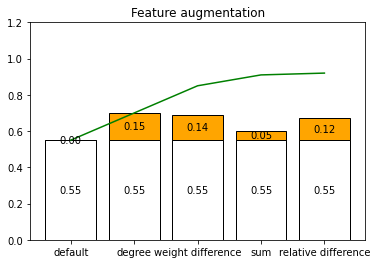
\includegraphics[scale=0.8]{figures/FeatureAugmentationLine}
    \caption{MNIST trained model. Average performance on 100 MNIST graphs}
    \label{Feature Augmentation Effect}
\end{figure}

The figure \ref{Feature Augmentation Effect} shows each feature's impact on performance. The default white column demonstrates the model's performance without any additional features. The green colored columns visualize the positive effect of adding a feature, while the last column represents the final result when all the features are added simultaneously. We can observe that every feature has a positive effect on the performance and gives the largest improvement so far compared to the other experiments.

With the features added to the nodes, we proceed to experiment with the aggregation functions for the message passing. In the table \ref{aggrtable} one can see how the performance changes depending on the aggregation function used.

\begin{table}[h!]
\centering
\begin{tabular}{|| c | c ||} 
 \hline
 Aggregation function & Performance compared to greedy \\ [0.5ex] 
 \hline\hline
 add & 92.0\% \\
 \hline
 sum & 89.5\% \\
 \hline
 mean & 90.2\% \\
 \hline
 min & 87.0\% \\
 \hline
 max & 94.4\% \\
 \hline
\end{tabular}
\caption{Aggregation function performance}
\label{aggrtable}
\end{table}

With fine-tuning of the models' hyperparameters and architecture, and augmenting node features having the most effect on the performance, results were moving closer to being reasonable. At this point, a full training set can be used to see more realistic results. The results were relatively promising, but further testing showed that, unfortunately, line graph transformation on large and dense enough graphs turned out to grow out of proportions and take too much time to process. Therefore, another architecture was considered.

\section{Edge prediction model}

Instead of turning edges to nodes, a model can give predictions on the edges directly. With this approach there is less preprocessing needed, but the model now needs to have extra layers for the edge prediction part of the model. The purpose of these layers is to classify the edges based on the embeddings produced by the initial model, this is described in more detail in the \hyperref[sec:architecture]{Architecture section}.

After training both the edge classification model and the line graph model on the 55000 MNIST graphs with the best hyperparameters discovered in previous section, the following results compared to the greedy algorithm were recorded: 101\% for edge classification and 103\% for line graph model.

The figure \ref{Model performance on MNIST} depicts how MNIST trained line graph and edge prediction model's compare in terms of performance on unseen MNIST graphs. The orange section of the bar represents the portion of the total weight that stemmed from the greedy algorithm solving the unsolved remains of the graphs.
\begin{figure}[H]
    \centering
    \hspace*{-2cm}
    \includegraphics[scale=1.0]{figures/LineVSEdgeOnMNIST}
    \caption{MNIST performance comparison}
    \label{Model performance on MNIST}
\end{figure}

Edge classification showed a slightly worse results on average than the line graph. In theory, this can be due to the line graph containing more structural information in it compared to the original one. Regardless of the slightly worse result, the edge classification approach was still favorable due to the large time consumption of the line graph conversion. Overall, the results themselves are rather promising. Both models manage to beat the greedy algorithm even when the greedy result is close to the optimal. However, running time was still a problem. Due to the small size of MNIST graphs, finding an optimal solution using the Blossom algorithm takes less time than using our \gls{gnn} model, because of the overhead computations needed for the neural network during the prediction phase, but the model should be able to catch up time-wise when given larger graphs. There is still the question of whether training on small graphs can help with larger graphs. The next step is to test the current model on a different graph - Cage10 from SuiteSparse. Cage10 is a graph with 11000 nodes and 100 000 edges. The results can be seen in figure \ref{model performance}:

\begin{figure}[H]
    \centering
    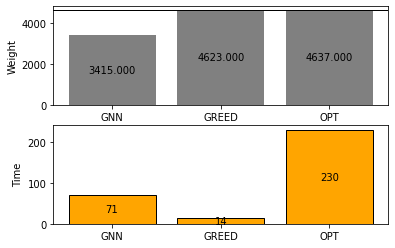
\includegraphics[scale=1.0]{figures/MNISTtrainCAGE10}
    \caption{MNIST trained model performance on cage10 graph}
    \label{model performance}
\end{figure}

As seen in figure \ref{model performance} the \gls{gnn} model manages to beat the optimal solver in terms of time, but it is noticeably worse in terms of total weight. Poor performance can be caused by the current training dataset. One of the main interests of the study was to see if the \gls{gnn} could be used on graphs larger than the ones it was trained on. It could be that the model fails to learn what is needed for larger graphs. Another reason could be that MNIST graphs have similar structures without enough variety to cover other graph types. One, of course, cannot include all the possible graphs in the training set, but the more data and variety the model gets during training the better. Therefore, another dataset was tried for training. A custom dataset consisting of randomly picked graphs from the SuiteSparse database. This custom dataset consists of 1000+ graphs with varying sizes and structures, between 100 and 10000 nodes.

Training the same model on the new dataset showed that the model struggled to learn the patterns. The flat information loss during training indicated that the model had a hard time learning the more diverse collection of graphs. Adding another layer to the classifier module of the model helped with a stagnating learning curve. Adding even more layers did not give any noticeable difference like adding the first layer did. A slightly deeper than the previous model gave the following results on the new dataset:

\begin{figure}[H]
    \centering
    \hspace*{-2cm}
    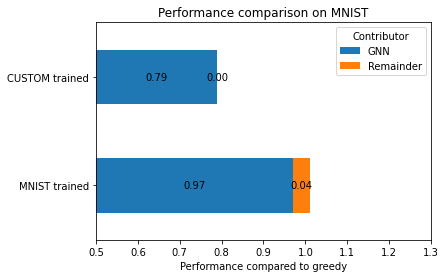
\includegraphics[scale=1.0]{figures/MNISTvsCUSTOMonMNIST}
    \caption{MNIST vs CUSTOM dataset training model performance on MNIST graphs}
    \label{models performance comparison}
\end{figure}

As partially expected, the model trained using custom datasets performed noticeably worse than the model trained on exclusively MNIST graphs. The custom dataset had both fewer and larger graphs than the ones in the MNIST dataset. This could be improved by adding some MNIST graphs to the custom dataset, but the main goal now is to see if the new dataset helps to get better performance on larger graphs. 

\begin{figure}[H]
    \centering
    \hspace*{-2cm}
    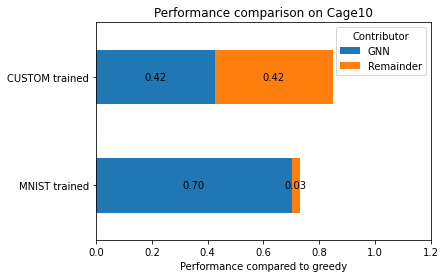
\includegraphics[scale=1.0]{figures/MNSITvsCUSTOMonCage10}
    \caption{MNIST vs CUSTOM dataset training model performance on cage10}
    \label{models performance comparison}
\end{figure}

\begin{figure}[H]
    \centering
    \includegraphics[scale=1.0]{figures/CUSTOMtrainCAGE10}
    \caption{CUSTOM trained model performance on cage10 graph}
    \label{model performance}
\end{figure}

The custom trained model does perform better in this case. However, it is not necessarily the model's accuracy itself that is the reason for improvement. The model seems to be rather indecisive on which nodes to match and half of the graph at the end is left unmatched, as opposed to the MNIST trained model matching almost the whole graph itself. This does, however, spark an idea that one might use the model to only match the most important nodes with the highest probabilities and leave the rest to the greedy algorithm to achieve better results. 

Results are still unsatisfying and there are a couple other ideas left to try: adjusting the matching threshold for the model and applying reduction.

\subsection{Reduction}

Reduction rules are used in algorithms to cut down the size of the graphs by removing the the parts of the graph are either guaranteed to be in the solution or the opposite. In the case of \gls{mwm}, it is the edges that must be included in the solution regardless. Ideally, the neural network should be able to pick up such edges by itself, but it is still worth testing to see if there is any positive effect as well as see if the model manages to grasp such rules by itself. The reduction rule itself is rather simple. If two connected nodes have an edge with a weight larger than the weight of the largest outgoing edge of each node, there is no reason not to pick it, since it is impossible to get a larger weight from these nodes. Figure \ref{Reduction example} serves as an example, where it is clear that node one should be matched with node five, if not, one has to match both one and five to other nodes. Second-best matchings for both node one and five have $weight = 3$, giving a total weight of only six.

\begin{comment}
\begin{algorithmic}[H]
\KwData{$graph G$}
\ForAll{$edge e$}
	\If{$e.weight > weight sum of largest remaining edge weights of the nodes$}
		\STATE $Pick the edge$\;
	\EndIf
\EndFor
\end{algorithmic}
\end{comment}

\begin{figure}[H]
    \centering
    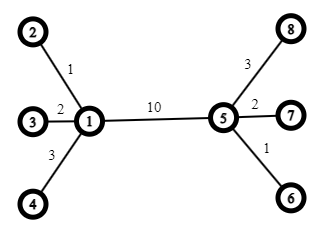
\includegraphics[scale=1.0]{figures/ReductionExample}
    \caption{Reduction example}
    \label{Reduction example}
\end{figure}

A couple of different graphs were used to test if the reduction helps and whether the model could find reducible edges on its own. In some cases there were graphs that had zero reducible edges, but in other cases such edges accounted for up to 5\% of the total number of edges. The model, however, did not seem to pick any of those edges in the graphs that contained the reducible edges on its own and adding reduction as a preprocessing step did improve the results by a small margin. Since the reduction is based on the heaviest edges of the nodes, it would make sense to add these node features to the model. 

The new model was trained with two additional node features: largest weight, second-largest weight for each node. Adding such features could in theory have helped the model to find reducible nodes, but after training the new model with the new node features the result, did not improve.

\subsection{Matching threshold}

Adjusting the threshold for picking the edges is another way to use the model. The model was initially set to consider all the edges that have a larger than 50\% chance of being in the solution. This matching threshold can be adjusted to, for example, only pick the edges with $90\%$ probability og being in the solution. This can help to focus the model on the edges that have a large impact on the total result, but would be otherwise ignored by a greedy algorithm. Additionally, it can be worth testing the removal of edges with low probabilities to see if the model can find edges that, if picked, inhibit the overall result.

\begin{figure}[H]
    \centering
    \hspace*{-1cm}
    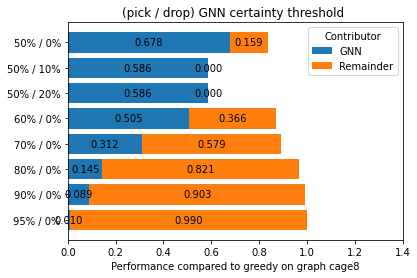
\includegraphics[scale=0.8]{figures/ThresholdDemo}
    \caption{Model threshold test on cage8 graph}
    \label{Model threshold test}
\end{figure}

Figure \ref{Model threshold test} shows how different thresholds affected the performance of the model. Remainder is solved by the greedy algorithm. The x-axis labels represent the thresholds for picking and dropping the edge respectively. For example, in the second column labeled “$50\% / 10\%$”, $50\%$ refers to the lowest prediction certainty required for an edge to be in the solution and $10\%$ refers to the edges with prediction certainty of being in the solution lower than $10\%$ to be removed from the graph comepletely.

The higher matching threshold does seem to improve the performance, but not enough to beat the greedy algorithm and most likely the increase is caused by the larger remainder being solved by th greedy algorithm due to fewer edges being above the threshold. Adding the drop threshold did not seem to work that well either. The model seems to assign very low scores to a lot of edges, which results in worse performance and no remainder for greedy algorithm to compensate. The reason for that is probably the weight class hyperparameter used during training, which makes the model care less for correctly finding nodes that should be ignored. The better approach could be to train the model specifically to find high value edges.

\section{Final results}

The final best model was tested on increasingly larger graphs from different sources. The final parameters of the model were:

\begin{enumerate}
\item Learning rate = $0.001$
\item Epochs = $300$
\item Mini-batch size = $1$
\item Network depth and width = $4$ layers, $640$ neurons each
\item Class weights = $0.1$ and $0.9$ for dropped and picked edges respectively
\item Weight decay = $0$
\item Match threshold = $70\%$
\item Added pre computed node features
	\begin{itemize}
	\item Degree - how many neighbours a node has.
	\item Sums of the weights. 	
	\item Weights sum relative to the neighbours.
	\item Weights sum difference compared to the neighbours.
	\end{itemize}
\item Agreggation function = Max
\end{enumerate}

\begin{figure}[H]
    \centering
    \hspace*{-2cm}
    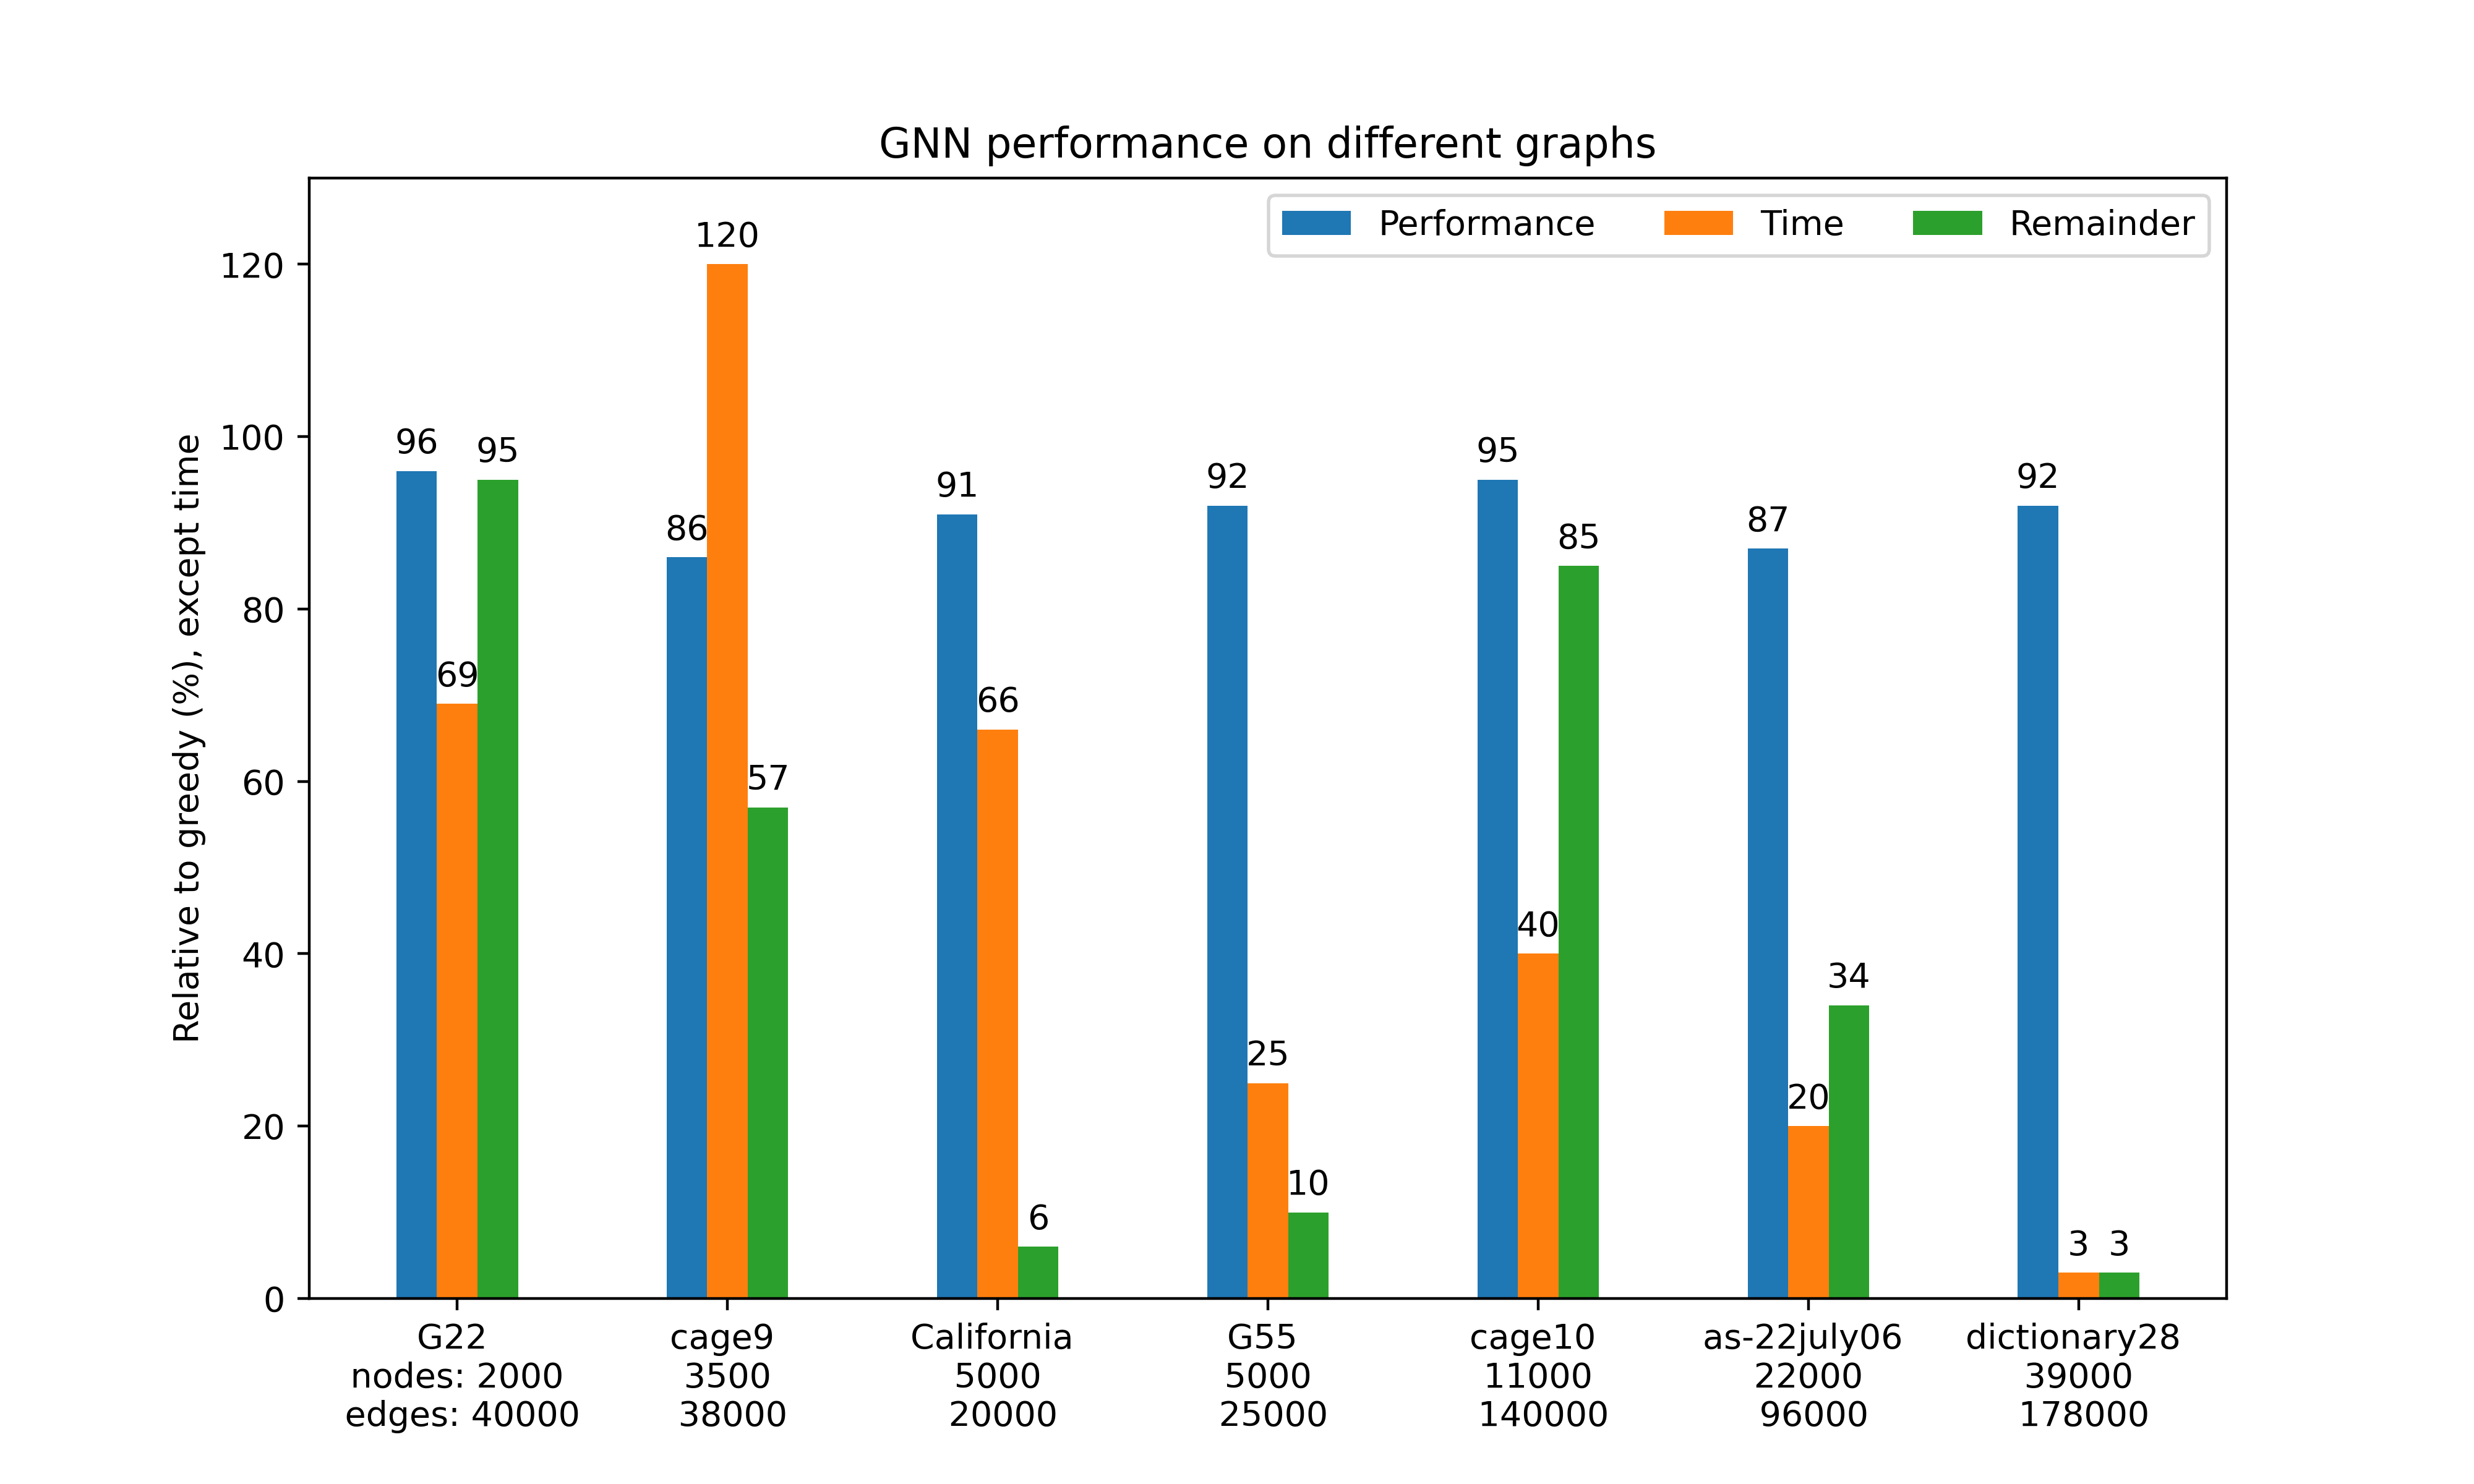
\includegraphics[scale=0.8]{figures/FINALResults}
    \caption{Final model performance}
    \label{Final model performance}
\end{figure}

Figure \ref{Final model performance} shows the performance of our final edge prediction model on the selection of increasingly larger graphs from different datasets. The blue colored columns stand for the models' performance on the graphs compared to the greedy algorithm. The green columns show the performance gained from solving the remainder of the graph with the greedy algorithm after the model could not find more edges. The orange column demonstrates the running time compared to the Blossom algorithm's running time.

Let's summarize the end results based on the main criteria.
\begin{itemize}
\item Performance: The total weight of the model's output seems to be rather stable at around 90\% of what a greedy algorithm produces, regardless of the size of the graph. It seems to be rather challenging for the model to beat the greedy approach when, in most cases, it makes up around 90-95\% of the total weight possible.
\item Running time: An exception in the sense that the time is shown in comparison to the time it takes to find the optimal solution. The reason for that is the fact that the model is always slower than the greedy algorithm. As expected, the benefit of using the \gls{gnn} can be seen as the size of the graphs increases. Smaller graphs take more time for the model to solve due to the overhead computations needed, but as the graphs grow the running time can get as small as 3\% of the Blossom algorithm.
\item Remainder: In some cases, the reason for the total weight being close to the greedy is the fact that the remainder makes up a large part of the graph, but it is not a consistent trend and neither does it depend on the size of the graph. There are cases with equally good results where the remainder is below 10\% of the total graph. The fact that some graphs leave such a big remainder indicates that the training dataset is not good enough and the model is not trained well enough to handle such graphs.
\end{itemize}

\subsection{Weakness of the greedy algorithm}
\label{sec:greedybadcase}
On average, a greedy algorithm seems to show good results, but in theory it is not hard to make a graph that abuses the greedy approach and results in poor performance. Example of a graph that \gls{gnn} model should be able to beat:

\begin{figure}[H]
    \centering
    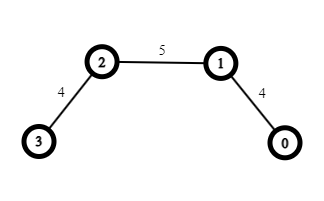
\includegraphics[scale=1.0]{figures/GoodCase}
    \caption{Good case for GNN}
    \label{Good case for GNN}
\end{figure}

In this very simple case, the greedy algorithm will result in total $weight = 5$. Yet the \gls{gnn} does manage to get the optimal $weight = 8$. This, of course, does not necessarily prove anything, but shows that there might be use cases for the model. There are more realistic graphs that the model also manages to solve better. 1138bus graph from SuitSparse is one of the examples where \gls{gnn} outperforms greedy by 15\%. Additionally, given that the running times of greedy and \gls{gnn} combined are still lower than the running time of finding the optimal solution, one may even run both and choose the better result.